% -*- latex -*-
%
% Copyright (c) 2002 The Trustees of Indiana University.  
%                    All rights reserved.
% 
% This file is part of the OSCAR software package.  For license
% information, see the COPYING file in the top level directory of the
% OSCAR source distribution.
%
% $Id: detailed.tex,v 1.64 2003/11/16 03:43:56 bernardli Exp $
%
% $COPYRIGHT$
%

\detailed{\section{Detailed Cluster Installation Procedure}}
\quick{\section{Quick Cluster Installation Procedure}}
\label{sec:detail}

All actions specified below should be performed by the \user{root}
user on the server node unless noted otherwise.  Note that if you
login as a regular user and use the \cmd{su} command to change to the
\user{root} user, you {\em must} use ``\cmd{su -}'' to get the full
\user{root} environment.  Using ``\cmd{su}'' (with no arguments) may
not be sufficient, and may cause obscure errors during an OSCAR
installation.

Note that all the steps below are mandatory unless explicitly marked
as optional.

\quick{Finally, note that this is specifically the ``Quick'' OSCAR
  installation guide.  There are a {\em lot} of details and
  explanations that are left out.  If you run into any problems or
  have any questions, please consult the complete OSCAR Installation
  Guide.}

%%%%%%%%%%%%%%%%%%%%%%%%%%%%%%%%%%%%%%%%%%%%%%%%%%%%%%%%%%%%%%%%%%%%%%%%%%
%%%%%%%%%%%%%%%%%%%%%%%%%%%%%%%%%%%%%%%%%%%%%%%%%%%%%%%%%%%%%%%%%%%%%%%%%%

\subsection{Server Installation and Configuration}
\label{det:serverinstall}
  
During this phase, you will prepare the machine to be used as the
server node in the OSCAR cluster.

%%%%%%%%%%%%%%%%%%%%%%%%%%%%%%%%%%%%%%%%%%%%%%%%%%%%%%%%%%%%%%%%%%%%%%%%%%

\subsubsection{Install Linux on the server machine} 
\label{det:serverosinstall}

If you have a machine you want to use that already has Linux
installed, ensure that it meets the minimum requirements as listed in
Section~\ref{sec:intro-min-sys}.  If it does, you may skip ahead to
Section~\ref{det:serverdiskpar}.

It should be noted that OSCAR is only supported on the distributions
listed in Table~\ref{tab:oscar-distro-support}
(page~\pageref{tab:oscar-distro-support}).  As such, use of
distributions other than those listed will likely require some porting
of OSCAR, as many of the scripts and software within OSCAR are
dependent on those distributions. 

\detailed{When installing Linux, it is not necessary to perform a
  ``custom'' install since OSCAR will usually install all the software
  on which it depends.  The main Linux installation requirement is
  that some X windowing environment such as GNOME or KDE must be
  installed.  Typically, a ``Workstation'' install with the ``Software
  Development Tools'' group added yields a sufficient installation for
  OSCAR to install successfully.}

It is best to {\em not} install distribution updates after you install
Linux; doing so may disrupt some of OSCAR's RPM dependencies.
Instead, install OSCAR first, and then install the distribution
updates.

%%%%%%%%%%%%%%%%%%%%%%%%%%%%%%%%%%%%%%%%%%%%%%%%%%%%%%%%%%%%%%%%%%%%%%%%%%

\subsubsection{Disk space and directory considerations}
\label{det:serverdiskpar}

OSCAR has certain requirements for server disk space. Space will be
needed to store the Linux RPMs and to store the images.  The RPMs will
be stored in \file{/tftpboot/rpm}.  2GB is usually enough to store the
RPMs.  The images are stored in \file{/var/lib/systemimager} and will
need approximately 2GB per image.  Although only one image is required
for OSCAR, you may want to create more images in the future.

\detailed{
  
  If you are installing a new server, it is suggested that you allow
  for 4GB in both the \file{/} (which contains \file{/tftpboot}) and
  \file{/var} filesystems when partitioning the disk on your server.

  If you are using an existing server, you will need to verify that
  you have enough space on the disk partitions.  Again 4GB of free
  space is recommended under each of \file{/} and \file{/var}.
  
  You can check the amount of free space on your drive's partitions by
  issuing the command \cmd{df -h} in a terminal.  The result for each
  file system is located below the \cmd{Available} column heading. If
  your root (\file{/}) partition has enough free space, enter the
  following command in a terminal:

  % Turns out that you can't put verbatim mode in \detailed{}.  Arrgh!

  {\tt \# mkdir -p /tftpboot/rpm}
  
  If your root partition does not have enough free space, create the
  directories on a different partition that does have enough free
  space and create symbolic links to them from the root (\file{/})
  directory.  For example, if the partition containing \file{/usr}
  contains enough space, you could do so by using the following
  commands:

  % Turns out that you can't put verbatim mode in \detailed{}.  Arrgh!

  {\tt \# mkdir -p /usr/tftpboot/rpm \\
    \indent \# ln -s /usr/tftpboot /tftpboot}
  
  The same procedure should be repeated for the
  \file{/var/lib/systemimager} subdirectory.

} % end detail

%%%%%%%%%%%%%%%%%%%%%%%%%%%%%%%%%%%%%%%%%%%%%%%%%%%%%%%%%%%%%%%%%%%%%%%%%%
    
\subsubsection{Download a copy of OSCAR and unpack on the server} 
\label{det:unpack}

If you are reading this, you probably already have a copy of an OSCAR
distribution package.  If not, go to
\url{http://oscar.sourceforge.net/} and download the latest OSCAR
Regular or Extra Crispy distribution package (see
Section~\ref{sec:download}, page~\pageref{sec:download}).  Ensure that
you have the latest documentation (later documentation may be
available on the OSCAR web site than in the OSCAR distribution
package).

Place the OSCAR distribution package in a directory such as
\user{root}'s home directory on the server node.  Although there is no
required installation directory (note that you may not use the
\begchange
directory \file{/usr/local/oscar}, \file{/opt/oscar}, 
\file{/var/lib/oscar}, or \file{/var/cache/oscar}  -- they are
reserved for use by OSCAR), the rest of these instructions will
\endchange
assume that you downloaded the OSCAR distribution package to
\user{root}'s home directory.

\detailed{
  
  Do {\bf not} unpack the tarball on a Windows-based machine and copy
  the directories over to the server, as this will convert all the
  scripts to ``DOS'' format and will render them useless under Linux.
  
  Open a command terminal and issue the following commands to unpack
  the OSCAR distribution package:

  % Turns out that you can't put verbatim mode in \detailed{}.  Arrgh!

  {\tt \# cd \\
    \indent \# tar zxf <filename>}
  
  Where \file{$<$filename$>$} is either
  \file{oscar-\oscarversion.tar.gz} (regular distribution) or
  \file{oscar\--including\--srpms\--\oscarversion.tar.gz} (extra
  crispy distribution).

  \def\obase{$^\sim$/oscar-\oscarversion}

  \begin{table}[htbp]
    \begin{center}
      \begin{tabular}{|l|p{3in}|}
        \hline
        \multicolumn{1}{|c|}{Directory} &
        \multicolumn{1}{|c|}{Contents} \\
        \hline
        \hline
        \file{\obase/} & the base OSCAR directory \\
                                %
        \file{\obase/COPYING} & GNU General Public License
        v2 \\
                                %
        \file{\obase/dist} & distribution scripts for configure/install \\
                                %
        \file{\obase/doc} & OSCAR documentation directory \\
                                %
        \file{\obase/images} & auxiliary images used in the GUI \\
                                %
        \file{\obase/install\_cluster} & main installation script \\
                                %
        \file{\obase/lib} & auxiliary library routines \\
                                %
        \file{\obase/oscarsamples} & sample configuration files \\
                                %
        \file{\obase/packages} & RPM and installation files for the
        OSCAR packages \\
                                %
        \file{\obase/README} & text README document \\
                                %
        \file{\obase/scripts} & contains scripts that do most of the
        work \\
                                %
        \file{\obase/share} & more auxiliary helper files \\
                                %
        \file{\obase/testing} & contains OSCAR cluster test helper
        scripts \\
                                %
        \file{\obase/VERSION} & file containing the OSCAR version number \\
        \hline
      \end{tabular}
      \caption{OSCAR distribution package file and directory layout.}
      \label{tab:oscar-dir-struct}
    \end{center}
  \end{table}
  
} % end detailed


%%%%%%%%%%%%%%%%%%%%%%%%%%%%%%%%%%%%%%%%%%%%%%%%%%%%%%%%%%%%%%%%%%%%%%%%%%

\subsubsection{Configure and Install OSCAR}
\label{det:configure-install}

%TJN: intentionally not using oscarversion 
Starting with OSCAR 2.3, after unpacking the tarball you will need to
configure and install OSCAR.  The configure portion sets up the release to
be permantently installed on the system in \file{/opt/oscar} (default
location).  The {\tt --prefix=\emph{ALT-DIR}} $\,$ flag can be used to
configure and install OSCAR into an alternate directory.  

The first step is to run the \file{configure} script, which is provided in
the top-level directory of the OSCAR release.  

  \vspace{11pt} {\tt
          \# cd /root/oscar-\oscarversion \\
  \indent \# ./configure }  \vspace{11pt} 

Once the configure script sucessfully completes you are ready to actually
install OSCAR on the server.  At this point no changes have been made to
the system beyond the \file{oscar-\oscarversion} directory itself.  Running
the following will copy the files to the system.  The files copied will
include the base OSCAR toolkit as well as startup scripts for the
\file{profile.d/} area.  The startup scripts add OSCAR to your path and set
environment variables like {\tt OSCAR\_HOME}.

  \vspace{11pt} {\tt
  \indent \# make install} \vspace{11pt}


At this point you will be ready to change to either the default
\file{/opt/oscar} directory or whatever path was use with the {\tt
--prefix} flag to perform the installation steps discussed in Section
\ref{det:installcluster}.
\begchange
  In the remainder of this document, the variable \file{\$OSCAR\_HOME} will
be used in place of the directory you installed OSCAR to -- by default
this is \file{/opt/oscar}.
\endchange


%%%%%%%%%%%%%%%%%%%%%%%%%%%%%%%%%%%%%%%%%%%%%%%%%%%%%%%%%%%%%%%%%%%%%%%%%%

\subsubsection{Configure the ethernet adapter for the cluster} 
\label{det:serveradapter}

Assuming you want your server to be connected to both a public
network and the private cluster subnet, you will need to have two
ethernet adapters installed in the server. This is the preferred OSCAR
configuration because exposing your cluster may be a security
risk and certain software used in OSCAR (such as DHCP) may conflict with
your external network.

Once both adapters have been physically installed in the server node,
you need to configure them.\footnote{Beware of certain models of 3COM
  network cards.  See footnote~\ref{foot:3com-warning} on
  page~\pageref{foot:3com-warning}.}  Any network configurator is
sufficient; popular applications include \cmd{neat}, \cmd{netcfg}, or
a text editor.

The following major requirements need to be satisfied:

\paragraph{Hostname.} Most Linux distributions default to the hostname
``{\tt localhost}'' (or ``{\tt localhost.localdomain}'').  This must
be changed in order to successfully install OSCAR -- choose another
name that does not include any underscores (``{\tt \_}'').

\paragraph{Public adapter.}  This is the adapter that connects the
server node to a public network.  Although it is not required to have
such an adapter, if you do have one, you must configure it as
appropriate for the public network (you may need to consult with your
network administrator).

\paragraph{Private adapter.}  This is the adapter connected to
the TCP/IP network with the rest of the cluster nodes.  This adapter
must be configured as follows:

\begin{itemize}
\item Use a private IP address\detailed{\footnote{There are three
      private IP address ranges: 10.0.0.0 to 10.255.255.255;
      172.16.0.0 to 172.32.255.255; and 192.168.0.0 to
      192.168.255.255.  Additional information on private intranets is
      available in RFC 1918.  You should not use the IP addresses
      10.0.0.0 or 172.16.0.0 or 192.168.0.0 for the server.  If you
      use one of these addresses, the network installs of the client
      nodes will fail.
    \label{foot:private-ip-ranges}}}

\item Use an appropriate netmask\detailed{\footnote{A class C netmask of
    255.255.255.0 should be sufficient for most OSCAR clusters.
    \label{foot:netmask}}}

\item Ensure that the interface is activated at boot time

\item Set the interface control protocol to ``none''

\end{itemize}

\detailed{
  
  Now reboot the server node to ensure that all the changes are
  propagated to the appropriate configuration files.  To confirm that
  all ethernet adapters are in the ``up'' state, once the machine has
  rebooted, open another terminal window and enter the following
  command:

  % Turns out that you can't put verbatim mode in \detailed{}.  Arrgh!

  {\tt \# ifconfig -a}
  
  You should see {\tt UP} as the first word on the third line of
  output for each adapter. If not, there is a problem that you need to
  resolve before continuing. Typically, the problem is that the wrong
  module is specified for the given device. Try using the network
  configuration utility again to resolve the problem.

} % end detailed
  
%%%%%%%%%%%%%%%%%%%%%%%%%%%%%%%%%%%%%%%%%%%%%%%%%%%%%%%%%%%%%%%%%%%%%%%%%%

\subsubsection{Copy distribution installation RPMs to \file{/tftpboot/rpm}}
\label{det:rpmcopy}

In this step, you need to copy the RPMs included with your Linux
distribution into the \file{/tftpboot/rpm} directory.  When each CD is
inserted, Linux usually automatically makes the contents of the CD be
available in the \file{/mnt/cdrom} directory (you may need to execute
a command such as ``\cmd{mount /mnt/cdrom}'' if the CD does not mount
automatically).

\detailed{
  
  For each CD, locate the directory that contains the RPMs.  In RedHat
  7.x, the RPMs are located in the \file{RedHat/RPMS} directory (i.e.,
  \file{/mnt/cdrom/RedHat/RPMS}).  Copy the RPMS into the
  \file{/tftpboot/rpm} directory with a command such as~\footnote{It may be
   helpful to use \cmd{rsync} for these mass copies to ensure the integrity of
   the data (at a cost of longer transfer times).  For example replace 
   the \cmd{cp} command in the example with \cmd{rsync -cav --stats}. }:

  % Turns out that you can't put verbatim mode in \detailed{}.  Arrgh!

  {\tt \# cp /mnt/cdrom/RedHat/RPMS/*.rpm /tftpboot/rpm}
  
  Be sure to repeat the above process for {\em all} CDs.  After using
  each CD you will have to unmount it from the local file system and
  eject it by issuing these commands:

  % Turns out that you can't put verbatim mode in \detailed{}.  Arrgh!

  {\tt \# cd \\
    \indent \# eject cdrom}

} % end detailed

%%%%%%%%%%%%%%%%%%%%%%%%%%%%%%%%%%%%%%%%%%%%%%%%%%%%%%%%%%%%%%%%%%%%%%%%%%

%\subsubsection{Copy distribution update RPMs to \file{/tftpboot/rpm}}
%\label{det:distro-updates}

%Obtain all the relevant RPM updates for your distribution -- security
%patches, bug fixes, etc.  Most distributions (including RedHat)
%include a tool to automate this process (e.g., \cmd{up2date}) that
%will automatically download and install all relevant updated RPMs.

%Ensure that these updated RPMs are also copied to
%\file{/tftpboot/rpm}.  It does not matter if two different versions of
%the same RPM end up in \file{/tftpboot/rpm} (e.g.,
%\file{foo-1.2.3-1.i386.rpm} from the installation CD and
%\file{foo-1.2.4-1.i386.rpm} from the updates) -- OSCAR will
%automatically use the latest version when it selects RPMs to install.


%%%%%%%%%%%%%%%%%%%%%%%%%%%%%%%%%%%%%%%%%%%%%%%%%%%%%%%%%%%%%%%%%%%%%%%%%%
%%%%%%%%%%%%%%%%%%%%%%%%%%%%%%%%%%%%%%%%%%%%%%%%%%%%%%%%%%%%%%%%%%%%%%%%%%
  
\subsection{Launching the OSCAR Installer}
\label{det:installcluster}

\quick{Run the \cmd{install\_\-cluster} script from OSCAR's top-level
  directory, with an argument specifying your server's private network
  adapter.  For example: \cmd{./install\_\-cluster eth0}.}

\detailed{
  
  Change directory to the top-level OSCAR directory and start the
  OSCAR install wizard:

% We have to use \tt instead of {verbatim} because we need to use
% \oscarversion inside.  This makes it somewhat painful -- much less
% easy than {verbatim}.
  \vspace{11pt} {\tt
\begchange
    \# cd \file{\$OSCAR\_HOME} \\
\endchange
    \indent \# ./install\_cluster $<$device$>$ } \vspace{11pt}
  
  In the above command, substitute the device name (e.g., \emph{eth1})
  in place of \cmd{$<$device$>$} for your server's private network
  ethernet adapter.  The script will execute some setup /
  configuration steps, including (but not limited to):

  \begin{enumerate}
  \item installs prerequisite packages on the server
  \item copies OSCAR RPMs to \file{/tftpboot/rpm}
  \item installs all OSCAR server RPMs
  \item updates \file{/etc/hosts} with OSCAR aliases
  \item updates \file{/etc/exports} 
  \item adds OSCAR paths to \file{/etc/profile} 
  \item updates system startup (\file{/etc/rc.d/init.d}) scripts
  \item restarts affected services
  \end{enumerate}
  
} % end detailed

A lot of output will be displayed in the console window where you
invoked \cmd{install\_cluster}.  This reflects normal operational
output from the various installation commands that OSCAR executes.
The output is also saved in the file \file{oscarinstall.log} for later
reference (particularly if something goes during during the
installation).
  
After the steps listed above have successfully finished, the OSCAR
installation wizard GUI will automatically be launched.
  
\detailed{
  
  The wizard, as shown in Figure~\ref{fig:detailed-oscar-wizard}, is
  provided to guide you through the rest of the cluster installation.
  To use the wizard, you will complete a series of steps, with each
  step being initiated by the pressing of a button on the wizard. Do
  not go on to the next step until the instructions say to do so, as
  there are times when you may need to complete an action outside of
  the wizard before continuing on with the next step. For each step,
  there is also a \button{Help} button located directly to the right
  of the step button.  When pressed, the \button{Help} button displays
  a message box describing the purpose of the step.

  \begin{figure}[htbp]
    \begin{center}
      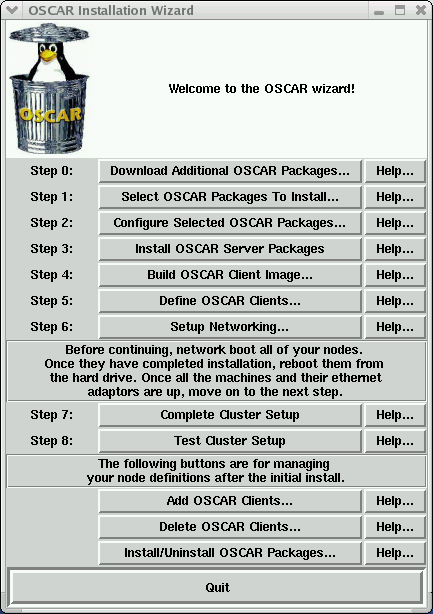
\includegraphics[scale=\imgscale]{figs/2_sbs-oscar-wizard}
      \caption{OSCAR Wizard.}
      \label{fig:detailed-oscar-wizard}
    \end{center}
  \end{figure}
  
} % end detailed
  
%%%%%%%%%%%%%%%%%%%%%%%%%%%%%%%%%%%%%%%%%%%%%%%%%%%%%%%%%%%%%%%%%%%%%%%%%%
%%%%%%%%%%%%%%%%%%%%%%%%%%%%%%%%%%%%%%%%%%%%%%%%%%%%%%%%%%%%%%%%%%%%%%%%%%

\subsection{Downloading Additional OSCAR Packages}
\label{det:opd}

\optional

The first step of the Wizard, ``Step 0'', enables you to download
additional packages.\footnote{Ganglia is a notable
  package that is not included in the main OSCAR distribution.  The
  process mentioned in this section will enable you to download
  Ganglia and install it with the rest of the OSCAR components.}  
The OSCAR Package Downloader (OPD) is a unified method of downloading
OSCAR packages and inserting them in the OSCAR installation hierarchy
so that they will be installed during the main OSCAR installation
process.  The Wizard uses a GUI frontend to OPD affectionately known as
\emph{OPDer}.  The addition of this frontend limits the need for direct
access to the command-line OPD tool directly.\footnote{Note, if using OPD
directly, the packages must be downloaded before the \button{Select OSCAR
Packages To Install} step (see Section~\ref{det:select-packages}) .}  
\begchange
If you would like to add additional repository URLs for testing
purposes, you can do this by accessing the \button{File} menu and then 
choosing \button{Additional Repositories...}. 
The remainder of this sub-section describes the underlying OPD tool.
\endchange

\quick{The command-line OPD can be launched outside of the GUI Wizard by 
  running the command \cmd{opd} from the top-level OSCAR \file{scripts} 
  directory.}

\detailed{
  The command-line OPD can be executed outside of the GUI Wizard from 
  the top-level OSCAR directory with the following command:

% We have to use \tt instead of {verbatim} because we need to use
% \oscarversion inside.  This makes it somewhat painful -- much less
% easy than {verbatim}.
  \vspace{11pt} {\tt
\begchange
    \indent \# cd \file{\$OSCAR\_HOME} \\
\endchange
    \indent \# ./scripts/opd } \vspace{11pt}
  
  OPD can use either the \cmd{wget} command or the built-in Perl LWP
  for downloading files.  By default, \cmd{wget} will be used if it
  can be found.  However, the use of LWP may be forced if the argument
  ``{\tt --lwp}'' is given on the command line.  LWP may be used in
  order to utilize a proxy, for example.  See the {\tt LWP::UserAgent}
  documentation for details on how to use proxies through LWP.

OPD requires some Perl modules to be installed before running.  If
they are not installed, you will receive a detailed error message
listing which modules need to be installed.  You have two options to
install these modules:

\begin{enumerate}
\item Use a tool such as CPAN to download and install the required
  modules.
  
\item Launch the OSCAR installer (see
  Section~\ref{det:installcluster}) and then quit immediately when the
  GUI window appears.  This is the preferred method, since the OSCAR
  installer will install of its own prerequisites (i.e., the process is
  automated).
\end{enumerate}

  
  Upon launching OPD, select a repository for packages from the
  choices listed.  OPD will then connect to that repository and query
  it for a list of available packages.  Select all the packages that
  you would like to download, and then use the ``download'' command to
  actually download them.
  
  Use the ``help'' command in OPD for listings of additional commands
  and help.

} % end detailed


%%%%%%%%%%%%%%%%%%%%%%%%%%%%%%%%%%%%%%%%%%%%%%%%%%%%%%%%%%%%%%%%%%%%%%%%%%
%%%%%%%%%%%%%%%%%%%%%%%%%%%%%%%%%%%%%%%%%%%%%%%%%%%%%%%%%%%%%%%%%%%%%%%%%%

\subsection{Selecting Packages to Install}
\label{det:select-packages}

\optional

If you wish to change the list of packages that are installed, click
on the \button{Select OSCAR Packages To Install} button.  This step is
optional -- by default all packages directly included in OSCAR are 
selected and installed.  However, if you downloaded any additional packages, 
e.g., via OPD/OPDer, they will not be selected for installation by default.  
Therefore you will need to click this button and select the appropriate OSCAR 
Packages to install on the cluster.

\detailed{
  
  When you click on the button, a window similar to the one shown in
  Figure~\ref{fig:detailed-package-selection} appears.  Each of the
  packages that the OSCAR installer has found are listed in the main
  frame. 
\begchange
  Core packages must be installed and cannot be unselected.  Included
  packages can be unselected if desired.
\endchange

  \begin{figure}[htbp]
    \begin{center}
      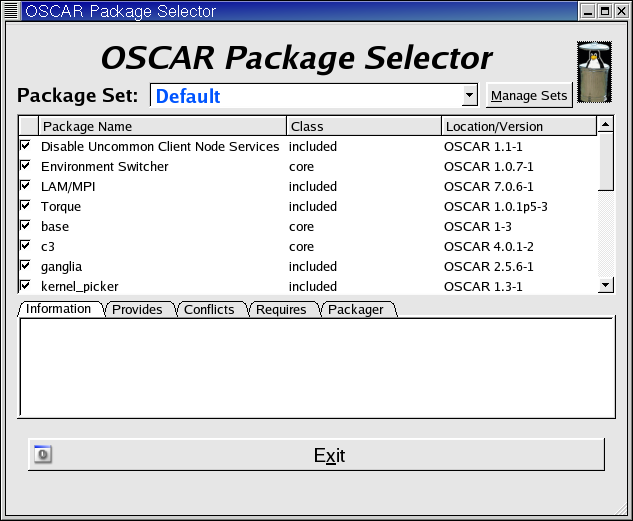
\includegraphics[scale=\imgscale]{figs/package-selection}
      \caption{OSCAR package selection.}
      \label{fig:detailed-package-selection}
    \end{center}
  \end{figure}
  
  Note that this window only shows {\em OSCAR packages} -- it does not
  show individual RPMs.
  
  Once you have a selected a set of OSCAR packages to install, click
\begchange
  on the \button{Exit} button to save your selections and
  return to the main OSCAR window.  Note that closing the window yields
  the same result and there is no way of `defaulting' to the original
  settings, so make sure your package list is complete before proceeding to 
  the next step.
\endchange

} % end detailed

%%%%%%%%%%%%%%%%%%%%%%%%%%%%%%%%%%%%%%%%%%%%%%%%%%%%%%%%%%%%%%%%%%%%%%%%%%
%%%%%%%%%%%%%%%%%%%%%%%%%%%%%%%%%%%%%%%%%%%%%%%%%%%%%%%%%%%%%%%%%%%%%%%%%%

\subsection{Configuring OSCAR Packages}
\label{det:configure-packages}

\optional

Some OSCAR packages allow themselves to be configured.  Clicking on
the \button{Configure Selected OSCAR Packages} button will bring up a
window listing all the packages that can be configured.
\detailed{Figure~\ref{fig:detailed-package-configuration} shows a
  sample with only the Environment Switcher package listed.}

\detailed{

  \begin{figure}[htbp]
    \begin{center}
      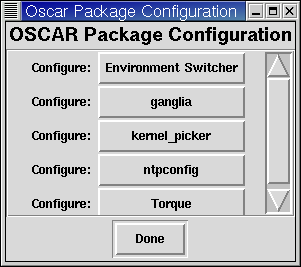
\includegraphics[scale=\imgscale]{figs/package-configuration}
      \caption{OSCAR package configuration.}
      \label{fig:detailed-package-configuration}
    \end{center}
  \end{figure}
  
  Clicking on any of the packages' \button{Config} button will bring
  up a panel for configuring that package.  Select whatever options
\begchange
  are appropriate for that package, and then click on the \button{Save}
  button to save your selections, or the \button{Cancel} button
  to cancel all of your selections and leave the original
  settings.  If you have saved your changes but want to go back to the
  default settings, simply click on the \button{Default Configuration} 
  button and then the \button{Save} button to revert to the original 
  settings.
\endchange  

  This step is optional.  If you do not click on the \button{Configure
    Selected OSCAR Packages} button, defaults for all packages will be
  used.

} % end detailed

%%%%%%%%%%%%%%%%%%%%%%%%%%%%%%%%%%%%%%%%%%%%%%%%%%%%%%%%%%%%%%%%%%%%%%%%%%

\subsubsection{Selecting a Default MPI Implementation}
\label{det:configure-packages-switcher}

Although multiple MPI implementations can be installed, only one can
be ``active'' for each user at a time.  Specifically, each user's path
needs to be set to refer to a ``default'' MPI that will be used for
all commands.  The Environment Switcher package provides a convenient
mechanism for switching between multiple MPI implementations.
\detailed{Section~\ref{app:switcher-which-mpi-to-use} contains more
  details about this package
  (page~\pageref{app:switcher-which-mpi-to-use}).}

The Environment Switcher package is mentioned now, however, because
its configuration panel allows you to select which MPI implementation
will be the initial ``default'' for all users.  OSCAR currently
includes two MPI implementations: LAM/MPI and MPICH.  Using
Environment Switcher's configuration panel, you can select one of
these two to be the cluster's default MPI.  

\detailed{
  
  You can change this default setting later -- see
  Section~\ref{app:switcher-which-mpi-to-use} for more details.
  
  When you close the main Configuration window, the following benign
  warning may appear in the shell window (it is safe to ignore):

  % Turns out that you can't put verbatim mode in \detailed{}.  Arrgh!

  {\tt Tag "mpi" does not seem to exist yet.  Skipping.}

} % end detailed

%%%%%%%%%%%%%%%%%%%%%%%%%%%%%%%%%%%%%%%%%%%%%%%%%%%%%%%%%%%%%%%%%%%%%%%%%%
%%%%%%%%%%%%%%%%%%%%%%%%%%%%%%%%%%%%%%%%%%%%%%%%%%%%%%%%%%%%%%%%%%%%%%%%%%

\subsection{Install OSCAR Server Packages}
\label{det:install-server-packages}

Press the \button{Install OSCAR Server Packages} button.  This will
invoke the installation of various RPMs and auxiliary configuration on
the server node.  Execution may take several minutes; text output
and status messages will appear in the shell window.

\detailed{
  
  A popup will appear indicating the success or failure of this step.
  Click on the \button{Close} button to dismiss it.

} % end detail

%%%%%%%%%%%%%%%%%%%%%%%%%%%%%%%%%%%%%%%%%%%%%%%%%%%%%%%%%%%%%%%%%%%%%%%%%%
%%%%%%%%%%%%%%%%%%%%%%%%%%%%%%%%%%%%%%%%%%%%%%%%%%%%%%%%%%%%%%%%%%%%%%%%%%

\subsection{Build OSCAR Client Image}
\label{det:build-client-image}

Before pressing the \button{Build OSCAR Client Image}, ensure that the
following conditions on the server are true:

\begin{itemize}

\item Ensure that the SSH daemon's configuration file
  (\file{/etc/ssh/sshd\_config}) on the headnode has {\tt PermitRootLogin} 
  set to {\tt yes}.  After the OSCAR installation, you may set this back 
  to {\tt no} (if you want), but it needs to be {\tt yes} during the install 
  because the config file is copied to the client nodes, and \user{root} 
  {\em must} be able to login to the client nodes remotely.

\item By the same token, ensure that TCP wrappers settings are not
  ``too tight''.  The \file{/etc/hosts.allow} and \file{/etc/hosts.deny} 
  files should allow all traffic from the entire private subnet.
  
\item Also, beware of firewall software that restricts traffic in the
  private subnet.
\end{itemize}

If these conditions are not met, the installation may fail during this
step or later steps.

Press the \button{Build OSCAR Client Image} button. A dialog will be
displayed. In most cases, the defaults will be sufficient. You should
verify that the disk partition file is the proper type for your client
nodes. The sample files have the disk type as the last part of the
filename. You may also want to change the post installation action and
the IP assignment methods.  \msg{It is important to note that if you
  wish to use automatic reboot, you should make sure the BIOS on each
  client is set to boot from the local hard drive before attempting a
  network boot by default. If you have to change the boot order to do
  a network boot before a disk boot to install your client machines,
  you should not use automatic reboot.}

\detailed{
  
  Building the image may take several minutes; the red progress bar on
  the bottom of the window will indicate how far along the process is.
  
  There is a lot of output in the console window during the build.  It
  is normal to see some warning messages in the console.  You can
  safely ignore these messages and wait for the final popup window
  announcing the success or failure of the overall image build.
  
  A sample dialog is shown in Figure~\ref{fig:detailed-build-image}.

  \begin{figure}[htbp]
    \begin{center}
      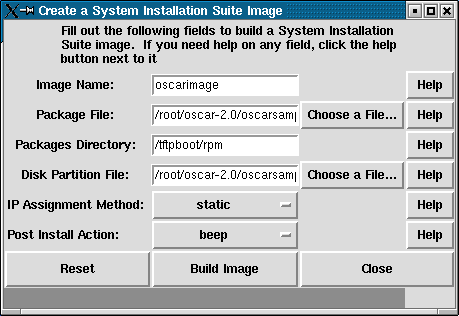
\includegraphics[scale=\imgscale]{figs/4a_sbs-build-image1}
      \caption{Build the image.}
      \label{fig:detailed-build-image}
    \end{center}
  \end{figure}

} % end detailed
  
\paragraph{Customizing your image.}
  
The defaults of this panel use the sample disk partition and RPM
package files that can be found in the \file{oscarsamples} directory.
You may want to customize these files to make the image suit your
particular requirements.

\subparagraph{Disk partitioning.}
  
The disk partition file contains a line for each partition desired,
where each line is in the following format:

\begin{verbatim}
  <partition> <size in megabytes> <type> <mount point> <options>
\end{verbatim}

\detailed{

  Here is a sample (for a SCSI disk):

% Actually include the real file so that we're never out of sync with
% what is shipped in the OSCAR distribution.

  \verbatiminput{../../oscarsamples/sample.disk.scsi}
  
  An * in the size column causes that partition to grow to fill the entire disk.  You
  can create your own partition files, but make sure that you do not
  exceed the physical capacity of your client hardware. Also be
  careful to not specify duplicate filesystems as this will cause
  problems during the installation. The sample listed above, and some
  others, are in the \file{oscarsamples} directory.

} % end detailed

\subparagraph{Package lists.}

The package list is simply a list of RPM file names (one per line). Be
sure to include all prerequisites that any packages you might add.
You do not need to specify the version, architecture, or extension of
the RPM filename.  For example, \file{bash-2.05-8.i386.rpm} need only
be listed as ``\file{bash}''.

\subparagraph{Custom kernels.}

If you want to use a customized kernel, you can add it to the image
after it is built (after installing the server OSCAR packages, but
before building the client image).  \detailed{See the
  \cmd{kernel\_\-picker} application description in
  Section~\ref{app:kernel-picker-overview} on
  page~\pageref{app:kernel-picker-overview}.}

\subparagraph{Build the Image.}

Once you are satisfied with the input, click the \button{Build Image}
button.  When the image completes, a popup window will appear
indicating whether the build succeeded or failed.  If successful,
click the \button{Close} button to close the popup, and then press the
\button{Close} button on the build image window.  You will be back at
the main OSCAR wizard menu.

\detailed{
  
  If the build fails, look through the console output\footnote{Note
    that all console output is also spooled into the file
    \file{oscarinstall.log}.} for some indication as to what happened
  to cause the failure.  Common causes include: prerequisite failure,
  ran out of disk space, and missing package files.  Also see the
  Release Notes for this version of OSCAR in
  Section~\ref{sec:release-notes} (page~\pageref{sec:release-notes}).

} % end detail


%%%%%%%%%%%%%%%%%%%%%%%%%%%%%%%%%%%%%%%%%%%%%%%%%%%%%%%%%%%%%%%%%%%%%%%%%%
%%%%%%%%%%%%%%%%%%%%%%%%%%%%%%%%%%%%%%%%%%%%%%%%%%%%%%%%%%%%%%%%%%%%%%%%%%

\subsection{Define OSCAR Clients}
\label{det:define-clients}

Press the \button{Define OSCAR Clients} button.  In the dialog box
that is displayed, enter the appropriate information.  Although the
defaults will be sufficient for most cases, you will need to enter a
value in the \field{Number of Hosts} field to specify how many clients
you want to create.

\begin{enumerate}
  
\item The \field{Image Name} field should specify the image name that
  was used to create the image in the previous step.
  
\item The \field{Domain Name} field should be used to specify the
  client's IP domain name.  
%
  It should contain the server node's domain (if it has one); if the
  server does not have a domain name, the default name
  \hostname{oscardomain} will be put in the field (although you may
  change it).
%
  {\bf This field \emph{must} have a value -- it cannot be blank.}
%
  \detailed{Note that especially for compute nodes on a private
    network, the domain name does not necessarily matter much.  The
    domain name supplied in this field is used to form the
    fully-qualified name of each host in the OSCAR cluster.  For
    example: \hostname{oscarnode1.oscardomain},
    \hostname{oscarnode2.oscardomain}, etc.  If your compute nodes are
    on a public network, you may want to use the ``real'' domain name
    that is part of their fully-qualified domain names.}

\item The \field{Base name} field is used to specify the first part of
  the client name and hostname. It will have an index appended to the
  end of it. This name \emph{cannot} contain an underscore 
  character ``\_''.

\item The \field{Number of Hosts} field specifies how many clients to
  create.  {\bf This number must be greater than 0.}
  
\item The \field{Starting Number} specifies the index to append to the
  \field{Base Name} to derive the first client name. It will be
  incremented for each subsequent client.
  
\item The \field{Padding} specifies the number of digits to pad the client
names, e.g., 3 digits would yeild oscarnode001.  The default is 0 to have
no padding between base name and number (index).

\item The \field{Starting IP} specifies the IP address of the first
  client. It will be incremented for each subsequent client.
  \detailed{See Footnote~\ref{foot:private-ip-ranges} on
    page~\pageref{foot:private-ip-ranges} for more information on how
    to pick a starting IP address.}
  
  \detailed{Clients will be given IP addresses starting with this IP
    address, and incrementing by 1 for each successive client.  Ensure
    that the range of $[ starting\_ip, (starting\_ip + num\_clients)
    ]$ does not conflict with the IP addresses of any other nodes on
    your network.}
  
  {\bf IMPORTANT NOTE:} Be sure that the resulting range of IP
  addresses does {\em not} include typical broadcast addresses such as
  $X.Y.Z.255$!  If you have more hosts than will fit in a single
  address range, see the note at the end of this section about how to
  make multiple IP address ranges.
  
\item The \field{Subnet Mask} specifies the IP netmask for all
  clients.  \detailed{See Footnote~\ref{foot:netmask} on
    page~\pageref{foot:netmask} for more information on how to select
    a netmask for your cluster.}
  
\item The \field{Default Gateway} specifies the default route for all
  clients.

\end{enumerate}
  
\detailed{
  
  When finished entering information, press the \button{Addclients}
  button.  When those clients have been created in the database, a
  popup will appear indicating the completion status.  A
  sample dialog is shown in Figure~\ref{fig:detailed-define-clients}.

  \begin{figure}[htbp]
    \begin{center}
      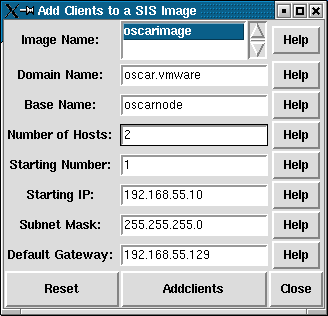
\includegraphics[scale=\imgscale]{figs/5a_sbs-define-clients1}
      \caption{Define the Clients.}
      \label{fig:detailed-define-clients}
    \end{center}
  \end{figure}
}

Note that this step can be executed multiple times.  The GUI panel
that is presented has limited flexibility in IP address numbering --
the starting IP address will only increment the least significant byte
by one for each successive client.  Hence, if you need to define more
than 254 clients (beware of broadcast addresses!), you will need to
run this step multiple times and change the starting IP address.
There is no need to close the panel and return to the main OSCAR menu
before executing it again; simply edit the information and click on
the \button{Addclients} button as many times as is required.

Additionally, you can run this step multiple times to use more
structured IP addressing schemes.  With a larger cluster, for example,
it may be desirable to assign IP addresses based on the top-level
switch that they are connected to.  For example, the 32 clients
connected to switch 1 should have an address of the form 192.168.1.x.
The next 32 clients will be connected to switch 2, and should
therefore have an address of the form 192.168.2.x.  And so on.

\detailed{After all clients have been created, you may press the
  \button{Close} button in the build clients dialogue and continue
  with the next step.}

%%%%%%%%%%%%%%%%%%%%%%%%%%%%%%%%%%%%%%%%%%%%%%%%%%%%%%%%%%%%%%%%%%%%%%%%%%
%%%%%%%%%%%%%%%%%%%%%%%%%%%%%%%%%%%%%%%%%%%%%%%%%%%%%%%%%%%%%%%%%%%%%%%%%%

\subsection{Setup Networking}
\label{det:setup-networking}

\detailed{
  
  The MAC address of a client is a twelve hex-digit hardware address
  embedded in the client's ethernet adapter. For example, ``{\tt
    00:0A:CC:01:02:03}'', as opposed to the familiar format of IP
  addresses.  These MAC addresses uniquely identify client machines on
  a network before they are assigned IP addresses. DHCP uses the MAC
  address to assign IP addresses to the clients.

} % end detail

In order to collect the MAC addresses, press the \button{Setup
  Networking} button. The OSCAR network utility dialog box will be
displayed.  To use this tool, you will need to know how to network
boot your client nodes, or have a file that lists all the MACs from
your cluster.  \detailed{For instructions on doing network booting,
  see Appendix~\ref{app:net-boot-client-nodes}. A sample dialog is
  shown in Figure~\ref{fig:detailed-collect-mac}.}

If you need to collect the MACs in your cluster, start the collection
by pressing the \button{Collect MAC Address} button and then network
boot the first client.  As the clients boot up, their MAC addresses
will show up in the left hand window. You have multiple options for
assigning MACs to nodes; you can either:

\begin{itemize}
\item manually select MAC address and the appropriate client in the
  right side window. Click \button{Assign MAC to Node} to associate
  that MAC address with that node.
  
\item click \button{Assign all MACs} button to assign all the MACs in
  the left hand window to all the open nodes in the right hand window.
\end{itemize}

\noindent Some notes that are relevant to collecting MAC addresses from the
network:

\begin{itemize}
\item The \button{Dynamic DHCP Update} checkbox at the bottom right of
  the window controls refreshing the DHCP server.  If it is selected
  (the default), the DHCP server configuration will be refreshed each
  time a MAC is assigned to a node.  Note that if the DHCP
  reconfiguration takes place quick enough, you may not need to reboot
  the nodes a second time (i.e., if the DHCP server answers the
  request quick enough, the node may start downloading its image
  immediately).
  
  If this option is off, you will need to click the \button{Configure
    DHCP Server} (at least once) to give it the associations between
  MACs and IP addresses.
  
\detailed {  
\item To remove extraneous MAC addresses from the left hand window
  (e.g., if the collector finds MACs that are not part of your
  cluster), select the address and click on the \button{Remove}
  button.  Or click on the \button{Remove All} button to remove all of
  them.

\item At any time, you may click on the \button{Export MACs to
    file...} button to save the MAC address list to a file.  If you
    need to re-run the OSCAR installation, you can later click on
    \button{Import MACs from file...} to import this file rather than
    re-collecting all the MACs.

\item When you have collected all of the MAC addresses, click the
  \button{Stop Collecting MACs} button.  If you do not have
  \button{Dynamic DHCP update} selected, you need to click the
  \button{Configure DHCP Server} button to configure the DHCP server.
}

\item You {\em must} click on the \button{Stop Collecting MACs} before
  closing the MAC Address Collection window!
\end{itemize}

You may also configure your remote boot method from this panel. The
\button{Build Autoinstall Floppy} button will build a boot floppy for
client nodes that do not support PXE booting. The \button{Setup
  Network Boot} button will configure the server to answer PXE boot
requests if your client hardware supports it. \detailed{See
  Appendix~\ref{app:net-boot-client-nodes} for more details.}

\detailed{
  
  When you have collected the addresses for all your client nodes and
  completed the networks setup, press the \button{Close} button.

  \begin{figure}[htbp]
    \begin{center}
      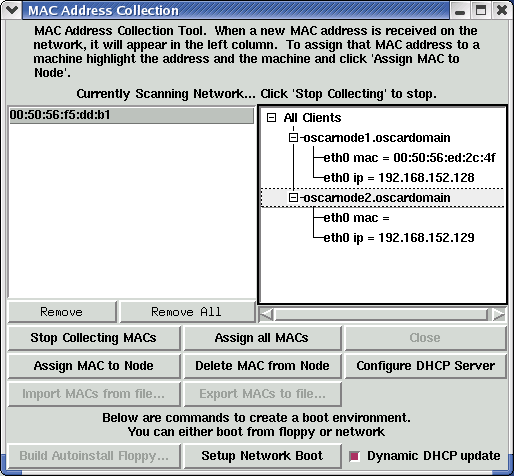
\includegraphics[scale=\imgscale]{figs/6e_sbs-found-mac}
      \caption{Collect client MAC addresses.}
      \label{fig:detailed-collect-mac}
    \end{center}
  \end{figure}

} % end detail

%%%%%%%%%%%%%%%%%%%%%%%%%%%%%%%%%%%%%%%%%%%%%%%%%%%%%%%%%%%%%%%%%%%%%%%%%%
%%%%%%%%%%%%%%%%%%%%%%%%%%%%%%%%%%%%%%%%%%%%%%%%%%%%%%%%%%%%%%%%%%%%%%%%%%

\subsection{Client Installations}
\label{det:client-install}

During this phase, you will network boot your client nodes and they
will automatically be installed and configured.  \detailed{For a
  detailed explanation of what happens during client installation, see
  Appendix~\ref{app:client-install}.}

%%%%%%%%%%%%%%%%%%%%%%%%%%%%%%%%%%%%%%%%%%%%%%%%%%%%%%%%%%%%%%%%%%%%%%%%%%

\subsubsection{Network boot the client nodes}

\detailed{See Appendix~\ref{app:net-boot-client-nodes} for
  instructions on network booting clients.}

Network boot all of your clients.  As each machine boots, it will
automatically start downloading and installing the OSCAR image from
the server node.

%%%%%%%%%%%%%%%%%%%%%%%%%%%%%%%%%%%%%%%%%%%%%%%%%%%%%%%%%%%%%%%%%%%%%%%%%%

\subsubsection{Check completion status of nodes}
\label{det:client-finish}

After several minutes, the clients should complete the installation.
You can watch the client consoles to monitor the progress. Depending
on the Post Installation Action you selected when building the image,
the clients will either halt, reboot, or beep incessantly when the
installation is completed.

\detailed{
  
  The time required for installation depends on the capabilities of
  your server, your clients, your network, and the number of
  simultaneous client installations.  Generally, it should complete
  within several minutes.

} % end detail
  
%%%%%%%%%%%%%%%%%%%%%%%%%%%%%%%%%%%%%%%%%%%%%%%%%%%%%%%%%%%%%%%%%%%%%%%%%%

\subsubsection{Reboot the client nodes}

After confirming that a client has completed its installation, you
should reboot the node from its hard drive. If you chose to have your
clients reboot after installation, they will do this on their
own. If the clients are not set to reboot, you must manually
reboot them. The filesystems will have been unmounted so it is safe
to simply reset or power cycle them.

\msg{Note: If you had to change the BIOS boot order on the client to
  do a network boot before booting from the local disk, you will need
  to reset the order to prevent the node from trying to do another
  network install.}

%%%%%%%%%%%%%%%%%%%%%%%%%%%%%%%%%%%%%%%%%%%%%%%%%%%%%%%%%%%%%%%%%%%%%%%%%%
%%%%%%%%%%%%%%%%%%%%%%%%%%%%%%%%%%%%%%%%%%%%%%%%%%%%%%%%%%%%%%%%%%%%%%%%%%

\subsection{Complete the Cluster Setup}
\label{det:complete-cluster-setup}

{\bf Ensure that all client nodes have fully booted before proceeding
  with this step.}

Press the \button{Complete Cluster Setup} button.  This will run the
final installation configurations scripts from each OSCAR software
package, and perform various cleanup and re-initialization functions.

\detailed{
  
  A popup window will indicate the success or failure of this step.
  Press the \button{Close} button to dismiss it.

} % end detail

%%%%%%%%%%%%%%%%%%%%%%%%%%%%%%%%%%%%%%%%%%%%%%%%%%%%%%%%%%%%%%%%%%%%%%%%%%
%%%%%%%%%%%%%%%%%%%%%%%%%%%%%%%%%%%%%%%%%%%%%%%%%%%%%%%%%%%%%%%%%%%%%%%%%%

\subsection{Test Cluster Setup}
\label{det:test-cluster}
            
A simplistic test suite is provided in OSCAR to ensure that the key
cluster components (OpenSSH, PBS, MPI, PVM, etc.) are functioning
properly.

Press the \button{Test Cluster Setup} button. This will open a
separate window to run the tests in.  The cluster's basic services are
checked and then a set of \user{root} and user level tests are run.

\detailed{
  
  A sample dialog is shown in Figure~\ref{fig:detailed-setup-test}. If
  any of the test fail, then there may be problem with your
  installation.

  \begin{figure}[htbp]
    \begin{center}
      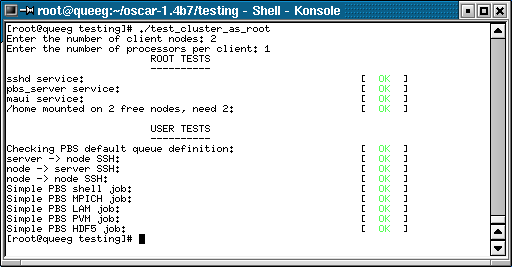
\includegraphics[scale=\imgscale]{figs/8_test-cluster-complete}
      \caption{Setup cluster tests}
      \label{fig:detailed-setup-test}
    \end{center}
  \end{figure}
  
  At the beginning of the test, when the PBS server is shut down, you
  may see a benign error message about the \cmd{pbsnodes} command not
  being able to connect to the PBS server.  This is safe to ignore.

} % end detail

%%%%%%%%%%%%%%%%%%%%%%%%%%%%%%%%%%%%%%%%%%%%%%%%%%%%%%%%%%%%%%%%%%%%%%%%%%
%%%%%%%%%%%%%%%%%%%%%%%%%%%%%%%%%%%%%%%%%%%%%%%%%%%%%%%%%%%%%%%%%%%%%%%%%%

\subsection{Congratulations!}

Your cluster setup is now complete. Your cluster nodes should
be ready for work.

\detailed{Be sure to read Section~\ref{sec:pkg-specific-notes}
  (starting on page~\pageref{sec:pkg-specific-notes}) -- it contains
  vital system administrator-level information on several of the
  individual packages that were installed as part of OSCAR.}

\quick{It is {\em strongly} recommended that you read the
  package-specific installation notes in the main Installation Guide.
  It contains vital system administrator-level information on several
  of the individual packages that were installed as part of OSCAR.}

%%%%%%%%%%%%%%%%%%%%%%%%%%%%%%%%%%%%%%%%%%%%%%%%%%%%%%%%%%%%%%%%%%%%%%%%%%
%%%%%%%%%%%%%%%%%%%%%%%%%%%%%%%%%%%%%%%%%%%%%%%%%%%%%%%%%%%%%%%%%%%%%%%%%%

\subsection{Adding and Deleting client nodes}

This section describes the steps need when it becomes necessary to add
or delete client nodes. If you have already built your cluster
successfully and would like to add or delete a client node, execute
the following from the top-level OSCAR directory:

\begin{verbatim}
  # ./install_cluster <device>
\end{verbatim}

\detailed{
  
  Like before, you must substitute the device name (e.g., \file{eth1})
  for the server node's internal ethernet adapter in the above
  command.  See Section~\ref{det:installcluster}
  (page~\pageref{det:installcluster}). Once the OSCAR wizard appears,
  you are ready to add or delete clients. Note that these steps will
  reuse the existing images made with the initial install, however, it
  will extend or contract the set of defined clients in the cluster.

} % end detail

%%%%%%%%%%%%%%%%%%%%%%%%%%%%%%%%%%%%%%%%%%%%%%%%%%%%%%%%%%%%%%%%%%%%%%%%%%

\subsubsection{Adding OSCAR clients}
\label{det:adding-clients}

Press the button of the wizard entitled \button{Add OSCAR Clients}.
\detailed{A sample dialog is shown in
  Figure~\ref{fig:detailed-add-node}.} These steps should seem
familiar -- they are same as the initial install steps.  Refer to
Sections~\ref{det:define-clients}, \ref{det:setup-networking}, and
\ref{det:complete-cluster-setup}.

Note that when adding nodes, in the Defining OSCAR Clients step, you
will typically need to change the following fields to suit your
particular configuration:

\begin{itemize}
\item Number of hosts
\item Starting number
\item Starting IP
\end{itemize}

\detailed{

  \begin{figure}[htbp]
    \begin{center}
      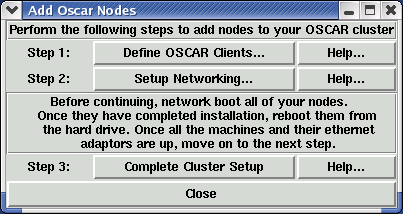
\includegraphics[scale=\imgscale]{figs/9a_sbs-add-node}
      \caption{Adding OSCAR clients.}
      \label{fig:detailed-add-node}
    \end{center}
  \end{figure}

} % end detail

%%%%%%%%%%%%%%%%%%%%%%%%%%%%%%%%%%%%%%%%%%%%%%%%%%%%%%%%%%%%%%%%%%%%%%%%%%

\subsubsection{Deleting clients}
\label{det:deleting-clients}

Press the button of the wizard entitled \button{Delete OSCAR Clients}.
\detailed{A sample dialog is shown in
  Figure~\ref{fig:detailed-delete-node}.}  Select the node(s) that you
wish to delete and press the button \button{Delete clients}, then
press \button{Close}.

\detailed{

  \begin{figure}[htbp]
    \begin{center}
      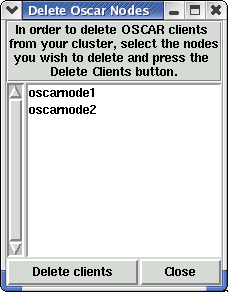
\includegraphics[scale=\imgscale]{figs/10a_sbs-del-node}
      \caption{Deleting OSCAR clients.}
      \label{fig:detailed-delete-node}
    \end{center}
  \end{figure}

} % end detail

%%%%%%%%%%%%%%%%%%%%%%%%%%%%%%%%%%%%%%%%%%%%%%%%%%%%%%%%%%%%%%%%%%%%%%%%%%
%%%%%%%%%%%%%%%%%%%%%%%%%%%%%%%%%%%%%%%%%%%%%%%%%%%%%%%%%%%%%%%%%%%%%%%%%%
\begchange
\subsection{Install/Uninstall OSCAR Packages}
\label{det:install-uninstall-packages}

The package installation system is a new feature in OSCAR 3.0 and is
designed to help simplify adding and removing OSCAR packages after the
initial system installaion.  The system is fairly straightforward for the
user as packages are selected for the appropriate action from the wizard.
This is the first release to support package install and uninstall from the
Wizard therefore some general background is provided to assist the user if
problems are encountered.

%%%%%%%%%%%%%%%%%%%%%%%%%%%%%%%%%%%%%%%%%%%%%%%%%%%%%%%%%%%%%%%%%%%%%%%%%%

\subsubsection{Selecting the Right Package}
\label{det:select-package}

Because of the way OSCAR handles packages, two packages of the same name
cannot currently c-exist nicely on the system.  Packages can be in one of
two spots:

\begin{enumerate}

\item \file{\$OSCAR\_HOME/packages} -- OSCAR installation directory
\item \file{/var/lib/oscar/package} -- OPD download area

\end{enumerate}

If there are multiple packages on the system of the same name, the package
located in the OPD download area is the package that the system recognizes.
It is possible that a package placed in /var/lib/oscar/package via a download
or manually could get loaded into the database, while the original package
that is located in \file{\$OSCAR\_HOME/packages} is the one that is actually
installed.  That is why this system does not support upgrades.  That is
planned for a future OSCAR release.  This can be avoided by uninstalling the
original package first before you download anything and then re-running the
wizard.  When the wizard first runs (\file{./install\_cluster ethX}), the
XML files are re-read for all packages and the database re-initialized.

%%%%%%%%%%%%%%%%%%%%%%%%%%%%%%%%%%%%%%%%%%%%%%%%%%%%%%%%%%%%%%%%%%%%%%%%%%

\subsubsection{Single Image Restriction}
\label{det:single-image-restriction}

Currently, if more than one image is detected on your system, the package
install/uninstall system will not run.  Packages are installed and
uninstalled to the clients (compute nodes), the server, and an image
(singular).  This release does not support the mapping of nodes to an
image for package install/uninstall through the wizard.  This single
image restriction is instituted to help reduce the risk of error with this
initial release, i.e., "keep it simpler".  The system looks for images in
\file{/var/lib/systemimager/images} and no other place.

%%%%%%%%%%%%%%%%%%%%%%%%%%%%%%%%%%%%%%%%%%%%%%%%%%%%%%%%%%%%%%%%%%%%%%%%%%

\subsubsection{Failures to Install and Uninstall}
\label{det:failures-install-uninstall}

A package is not installed or uninstalled until it successfully installs or
uninstalls on the compute nodes, the server, and a single image.  We will
run through an example problem as the best way of describing how to debug 
the system.  As a note, the system does sanity checking to try to avoid the
following situation.

For example, during the install process the clients may have been successfully
installed, but the server installation died half way through for some unknown
reason, and the install program exits with an error.  If this happens, a
second attempt to install will probably fail even if the server's problem
is resolved.

The reason for this is that something happened on the clients and it
succeeded, probably RPM's were installed.  So the second time you go to
install the package, the \file{rpm -Uvh} command on the nodes will fail.
A \file{-f} flag is avoided.

So, what do you do?

Really, you have two options.  The first is to look back through the log to
see what commands were run, and undo those commands by hand.  The second
would be to manually push out the uninstall scripts to the compute nodes,
and run them outside of the wizard environment.  All scripts are re-runnable
in OSCAR, and for serveral good reasons.

These options are not good ones, and we recognize this fact.  We are working
on better tools for general use.  Generally, it is a difficult problem to
judge error codes on remote systems and try to guess the appropriate actions
to take.  We have developed some additional software to start solving this
problem, but there is still work that needs to be done in this area.

On the uninstall side of things, the picture is much simpler.  The only
action taken by the system is to run the package's uninstall script and
judge the return code.  So an uninstall failure is probably a faulty
uninstall script.

%%%%%%%%%%%%%%%%%%%%%%%%%%%%%%%%%%%%%%%%%%%%%%%%%%%%%%%%%%%%%%%%%%%%%%%%%%

\subsubsection{More Debugging Info}
\label{det:more-debug-info}

Some amount of trouble was taken to insure that decent debugging output
was printed to the log -- making best use of this output is your best bet
in an error case.

\endchange 
%%%%%%%%%%%%%%%%%%%%%%%%%%%%%%%%%%%%%%%%%%%%%%%%%%%%%%%%%%%%%%%%%%%%%%%%%%
%%%%%%%%%%%%%%%%%%%%%%%%%%%%%%%%%%%%%%%%%%%%%%%%%%%%%%%%%%%%%%%%%%%%%%%%%%

\subsection{Starting over -- installing OSCAR again}

If you feel that you want to start the cluster installation process
over from scratch in order to recover from irresolvable errors, you
can do so with the \cmd{start\_over} script located in the
\file{scripts} subdirectory.

It is important to note that \cmd{start\_over} is {\em not} an
uninstaller.  That is, \cmd{start\_over} does {\em not} guarantee to
return the head node to the state that it was in before OSCAR was
installed.  It does a ``best attempt'' to do so, but the only
guarantee that it provides is that the head node will be suitable for
OSCAR re-installation.  For example, the RedHat 7.x series ships with
a LAM/MPI RPM.  The OSCAR install process removes this RedHat-default
RPM and installs a custom OSCAR-ized LAM/MPI RPM.  The
\cmd{start\_over} script only removes the OSCAR-ized LAM/MPI RPM -- it
does not re-install the RedHat-default LAM/MPI RPM.

Another important fact to note is that because of the environment
manipulation that was performed via \cmd{switcher} from the previous
OSCAR install, {\em it is necessary to re-install OSCAR from a shell
  that was not tainted by the previous OSCAR installation}.
Specifically, the \cmd{start\_over} script can remove most files and
packages that were installed by OSCAR, but it cannot chase down and
patch up any currently-running user environments that were tainted by
the OSCAR environment manipulation packages.

Ensuring to have an untainted environment can be done in one of two
ways:

\begin{enumerate}
\item After running \cmd{start\_over}, completely logout and log back
  in again before re-installing.  {\em Simply launching a new shell
    may not be sufficient} (e.g., if the parent environment was
  tainted by the previous OSCAR install).  This will completely erase
  the previous OSCAR installation's effect on the environment in all
  user shells, and establish a set of new, untainted user
  environments.
  
\item Use a shell that was established {\em before} the previous OSCAR
  installation was established.  Although perhaps not entirely
  intuitive, this may include the shell was that initially used to
  install the previous OSCAR installation.
\end{enumerate}

Note that the logout/login method is {\em strongly} encouraged, as it
may be difficult to otherwise absolutely guarantee that a given
shell/window has an untainted environment.

% LocalWords:  Exp
